\section{Results}
\subsection{Localization precision of the microscope}
A set of 100 images of the fluorescent 0.1 $\mu$m beads was acquired for each of the laser wavelengths.
An isolated bead was selected and its (two-dimensional) intensity profile was fitted in all images with a (two-dimensional) gaussian curve, using the \verb|curve_fit| \software{Scipy} function \hl{ici ou setup?}. 
The mean and standard variation of the resulting curve provide the $(x,y)$ localisation of the bead and the width of its PSF.
An example of the result of the localization, superimposed on one of the images acquired with the 647 nm laser, is depicted in \autoref{fig:beads_inset_zoom}.


\begin{figure}[htbp]
    \centering
    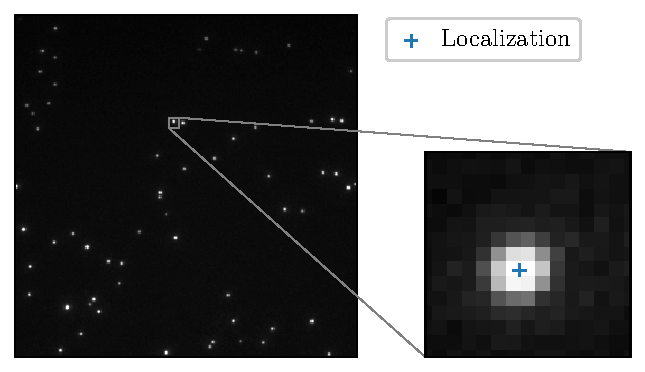
\includegraphics[scale=1]{figures/beads_inset_zoom.pdf}
    \caption{Whole acquisition (647 nm) and zoom on selected fluorescent bead.}
    \label{fig:beads_inset_zoom}
\end{figure}

\autoref{fig:comparison_wavelengths} compares the results [distributions of the $x$ and $y$ positions and their uncertainty] obtained with each laser wavelength.
DRIFTING ICI OU DISCUSSION? PEUT-ÊTRE ICI AVEC IMAGE

\begin{figure}[htbp]
    \begin{subfigure}{0.49\textwidth}
        \centering
        \fbox{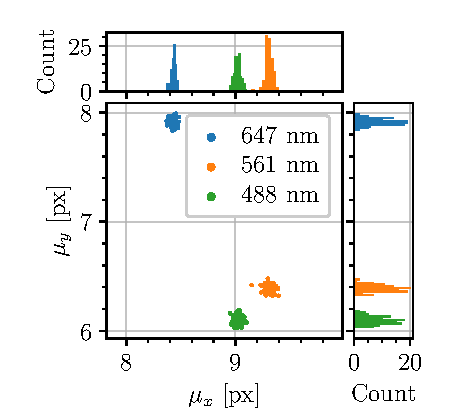
\includegraphics[scale=1]{figures/comparison_mu.pdf}}
        \caption{}
        \label{fig:comparison_mu}
    \end{subfigure}
    \begin{subfigure}{0.49\textwidth}
        \centering
        \fbox{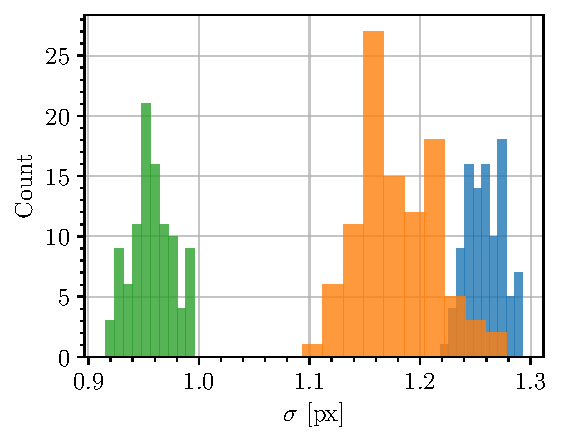
\includegraphics[scale=1]{figures/comparison_sigma.pdf}}
        \caption{}
        \label{fig:comparison_sigma}
    \end{subfigure}
    \caption{Comparison of (a) localisation position and (b) uncertainty distributions for the three different laser wavelengths.}
    \label{fig:comparison_wavelengths}
\end{figure}

Finally, the observed PSF widths were compared with the values expected for each wavelength from \autoref{eq:PSF_width_gaussian}.
As shown in \autoref{fig:comparison_PSF}, the PSF width computed is higher than the one expected.

\begin{figure}
    \centering
    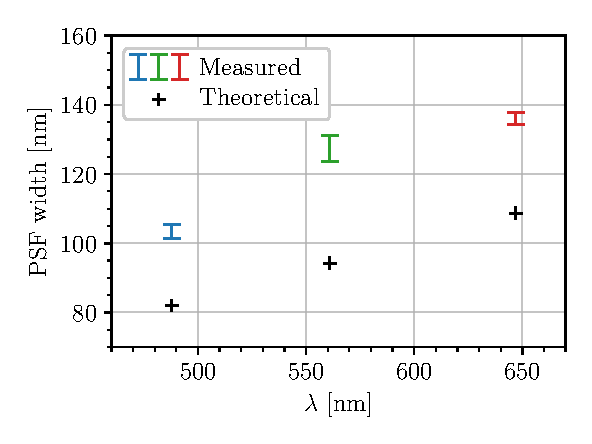
\includegraphics[scale=1]{figures/comparison_PSF.pdf}
    \caption{LABELS ET DIFFERENT COULEURS OU MARKER}
    \label{fig:comparison_PSF}
\end{figure}

\subsection{STORM imaging of micro-tubules}
\begin{figure}[htbp]
    \begin{subfigure}[b]{0.49\textwidth}    % trim left bottom right top
        \centering
        \raisebox{0.5cm}{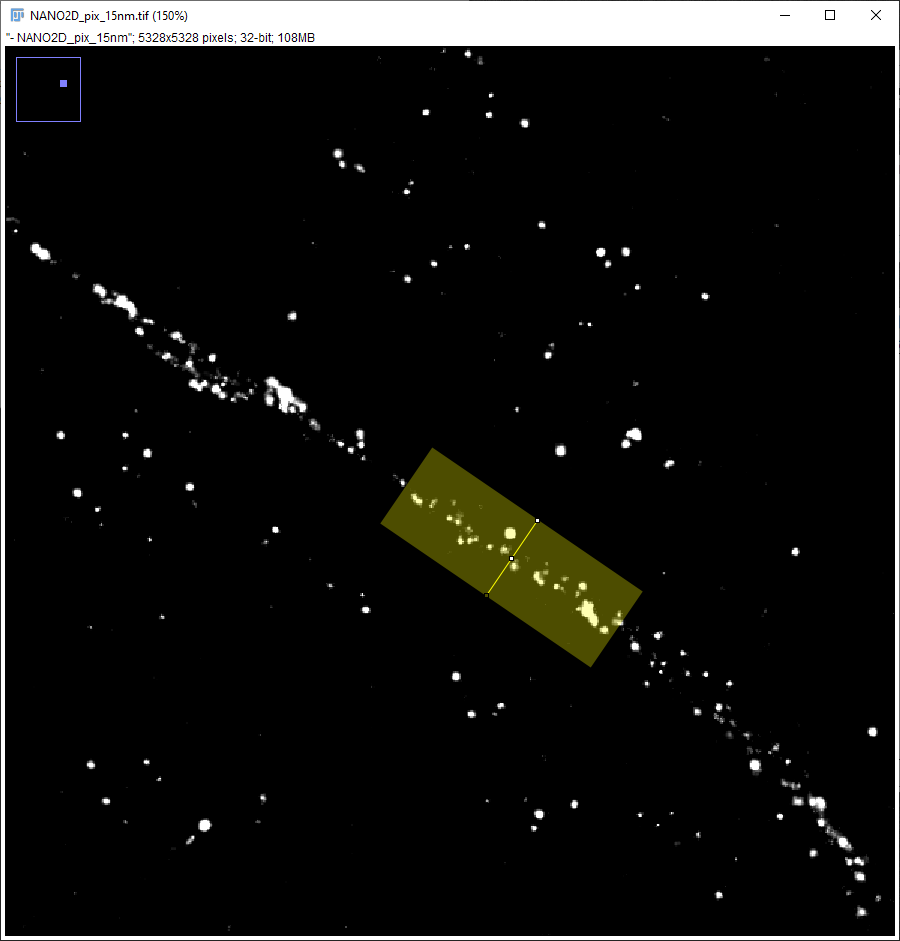
\includegraphics[width=0.9\textwidth, trim={1cm 1.5cm 1cm 5cm}, clip]{figures/microtubules_width_acquisition.PNG}}
        \caption{}
        \label{fig:microtubules_width_acquisition}
    \end{subfigure}
    \begin{subfigure}[b]{0.49\textwidth}
        \centering
        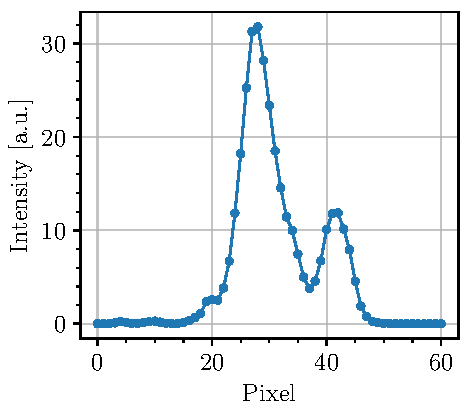
\includegraphics[scale=1]{figures/microtubules_width.pdf}
        \caption{}
        \label{fig:microtubules_width_analysis}
    \end{subfigure}
    \label{fig:microtubules_width}
    \caption{Intensity profile along a microtubule strand: (a) screen capture of the profile acquisition using the \software{Fiji} processing package, (b) the intensity profile averaged over the portion of length considered.}
\end{figure}

\begin{figure}
    \begin{subfigure}{0.32\textwidth}
        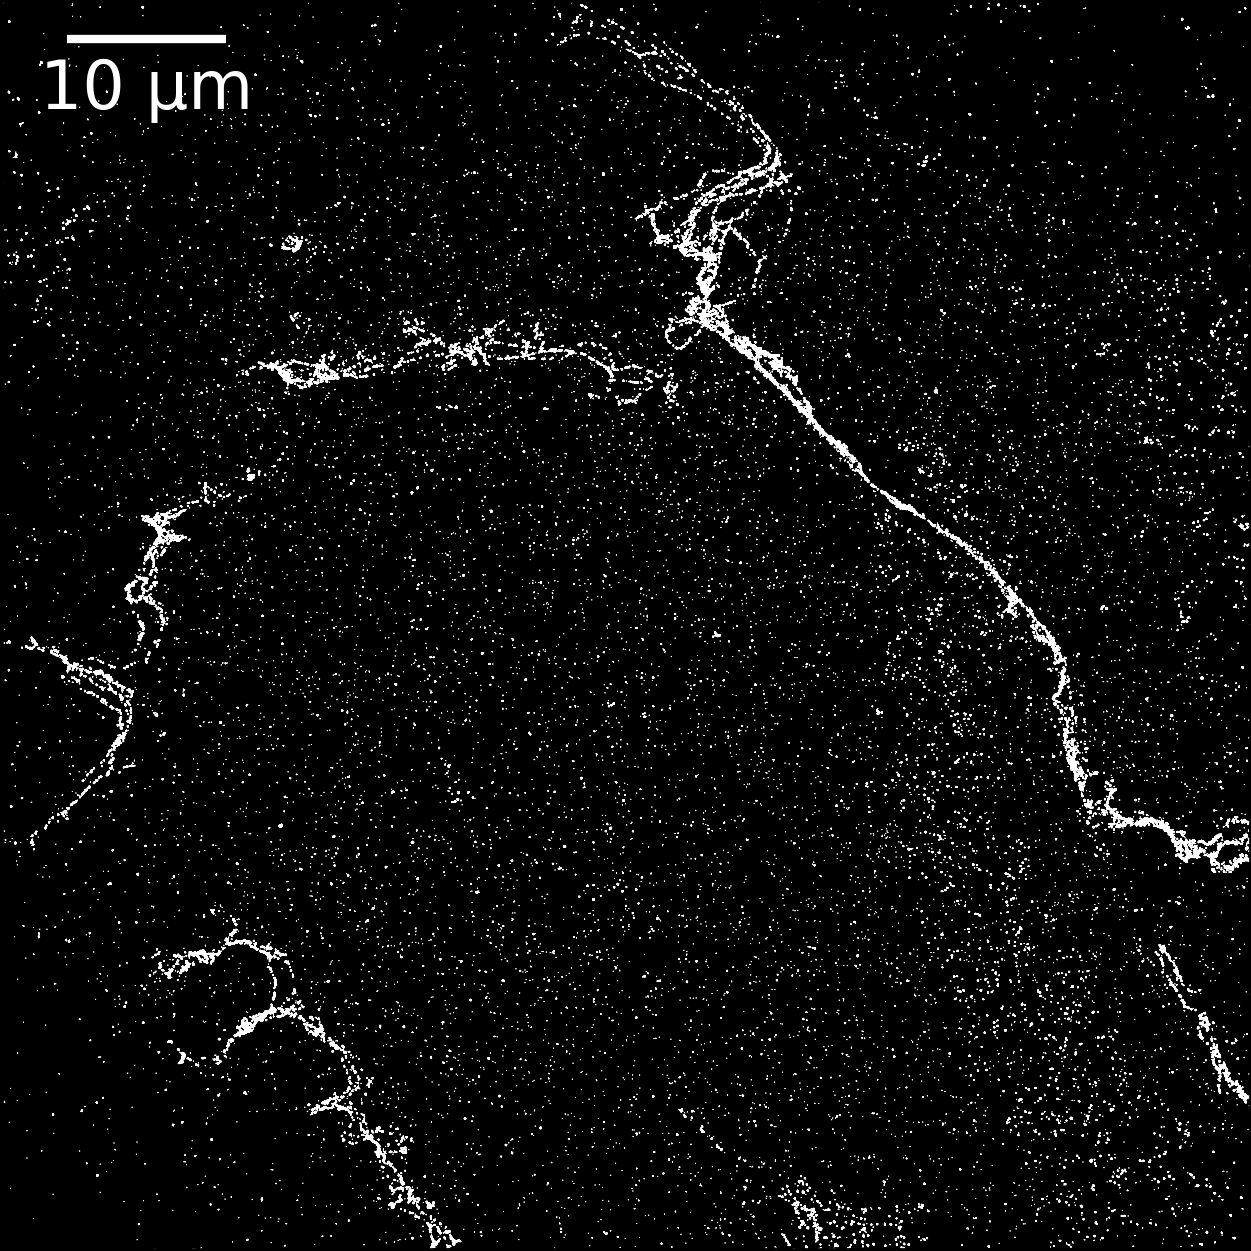
\includegraphics[width=\textwidth]{figures/microtubules_image1.png}
        \caption{}
    \end{subfigure}
    \begin{subfigure}{0.32\textwidth}
        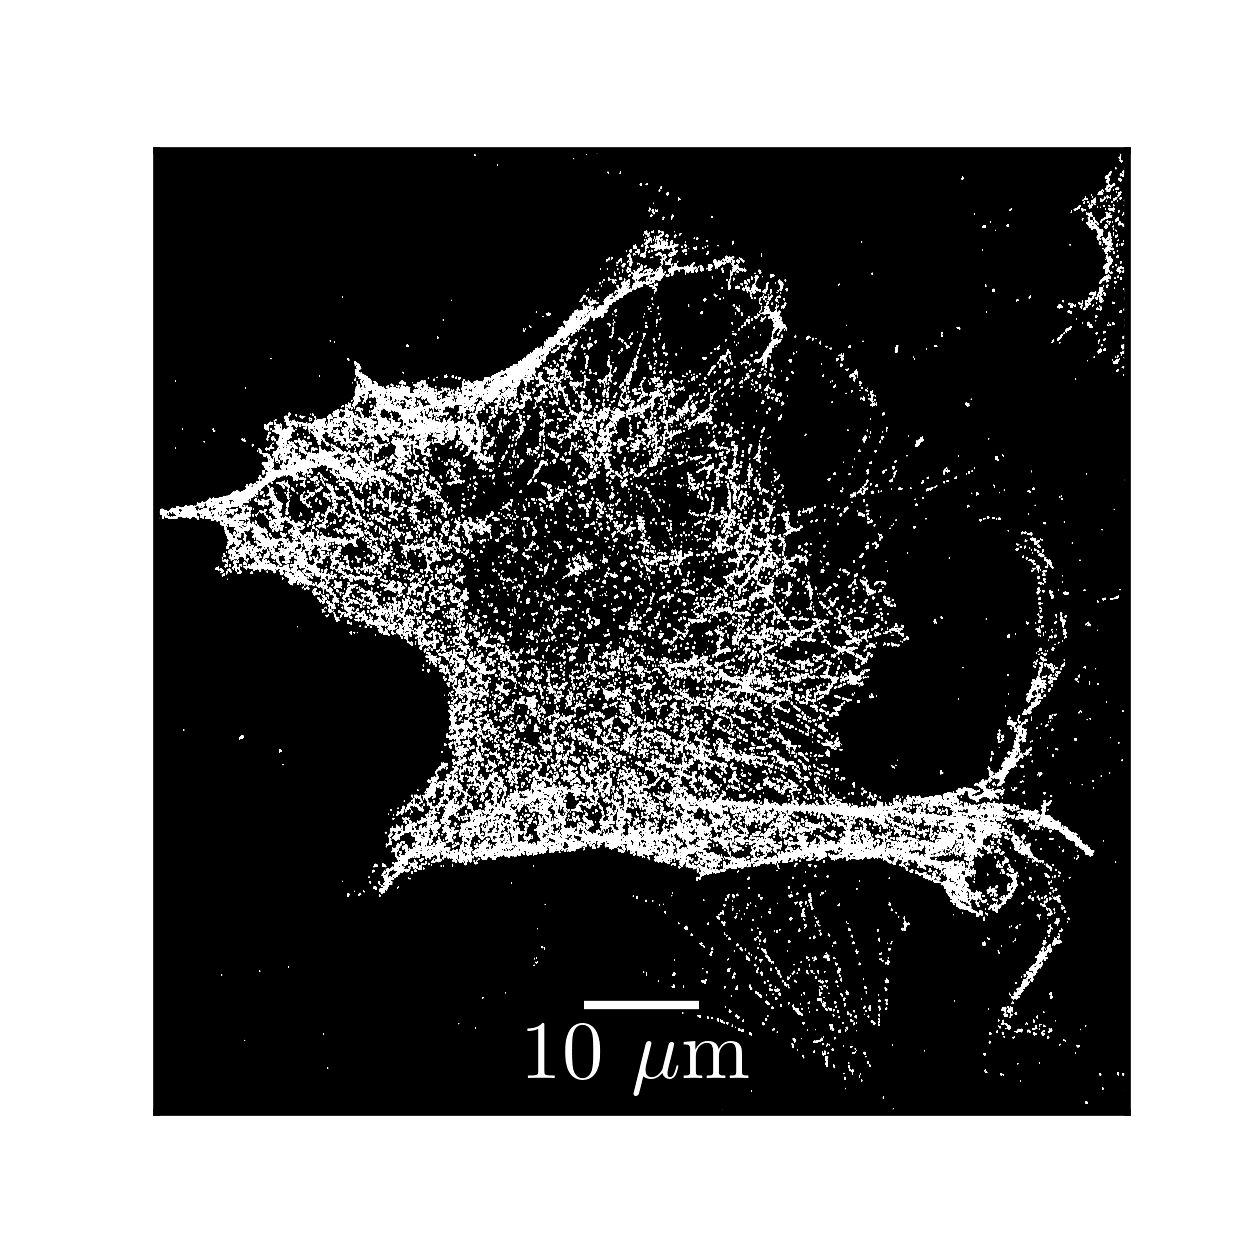
\includegraphics[width=\textwidth]{figures/microtubules_image4.png}
        \caption{}
    \end{subfigure}
    \begin{subfigure}{0.32\textwidth}
        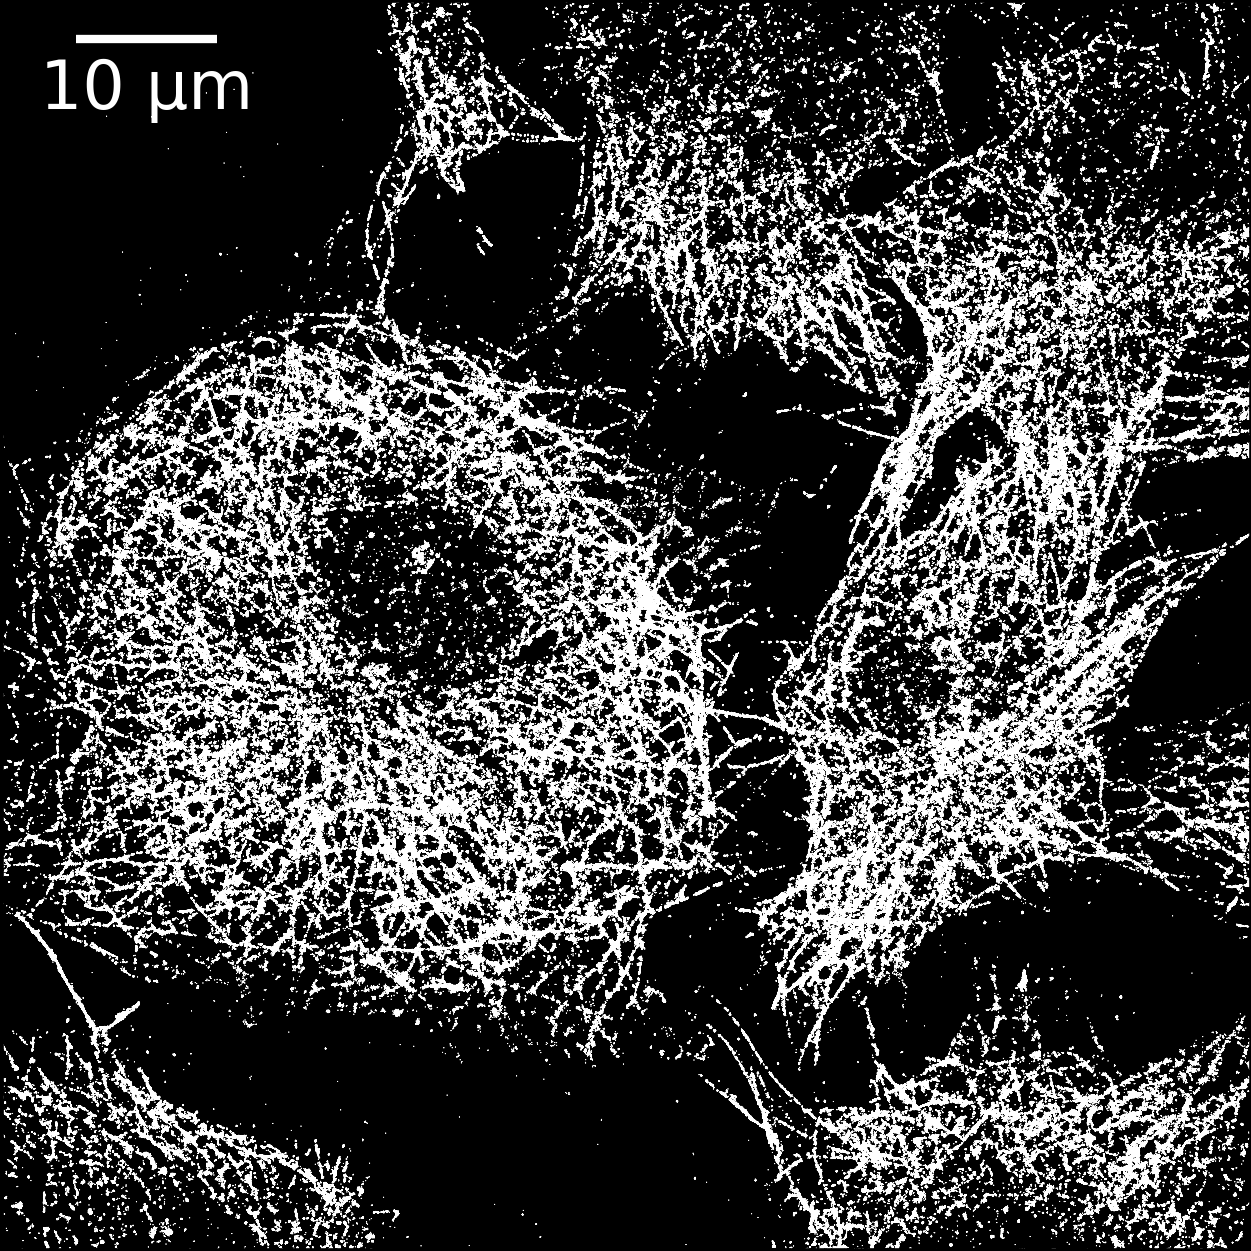
\includegraphics[width=\textwidth]{figures/microtubules_image6.png}
        \caption{}
    \end{subfigure}
    \caption{Micro-tubules}
\end{figure}

\subsection{Mitochondria}
\begin{figure}
    \begin{subfigure}{0.32\textwidth}
        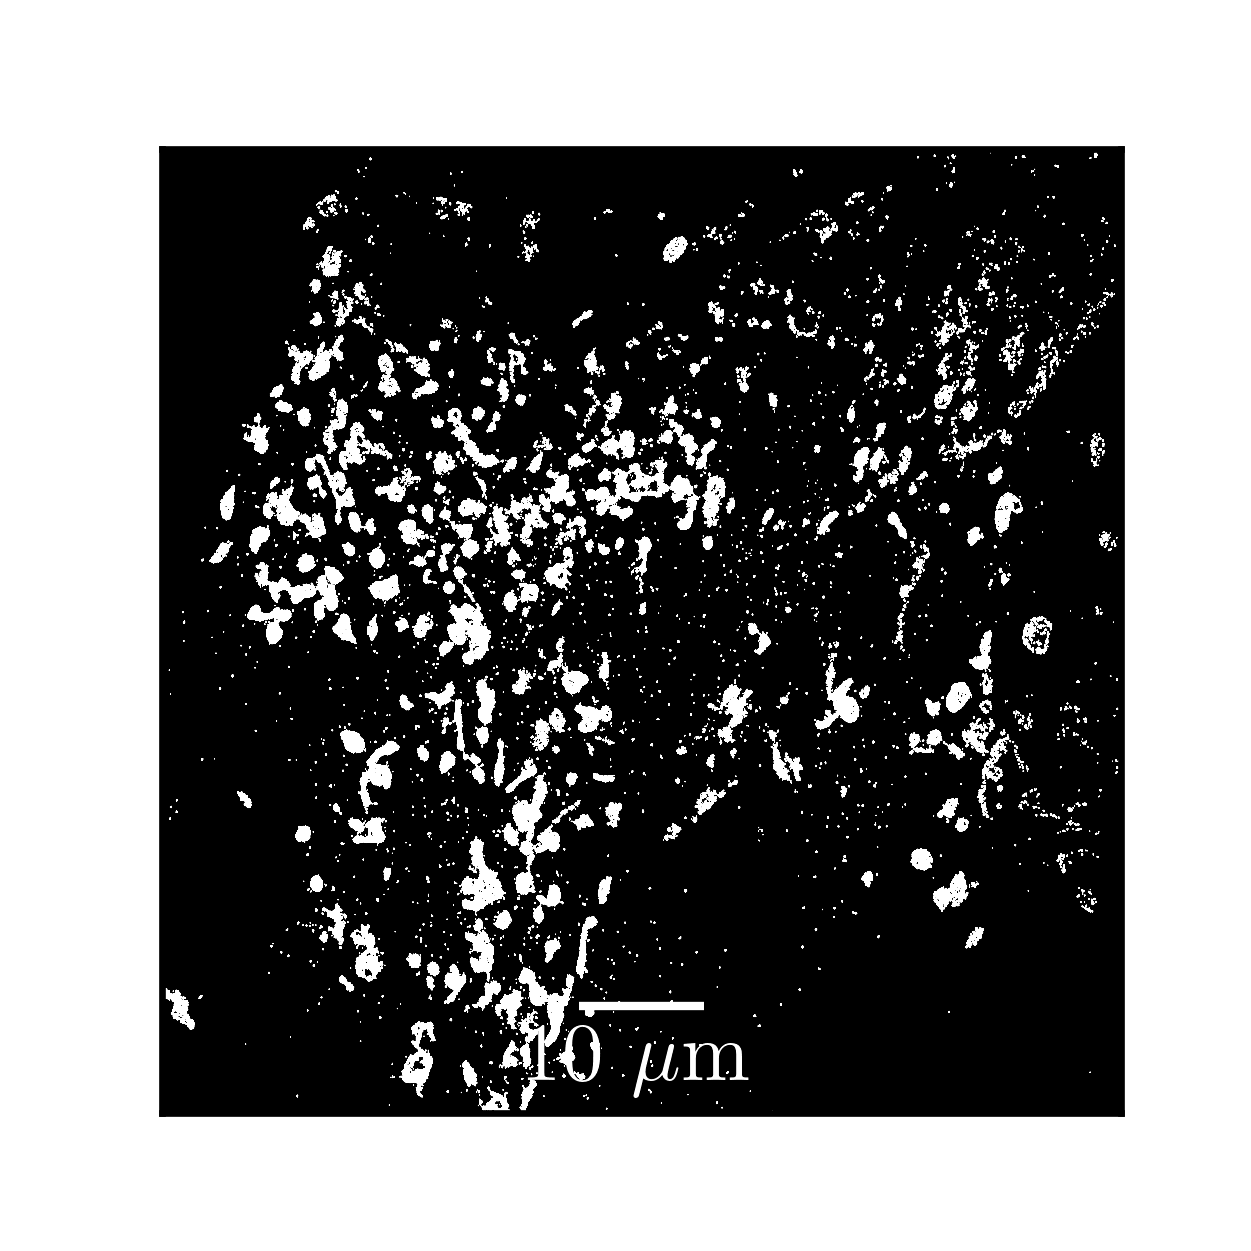
\includegraphics[width=\textwidth]{figures/mitochondria_image6.png}
        \caption{}
    \end{subfigure}
    \begin{subfigure}{0.32\textwidth}
        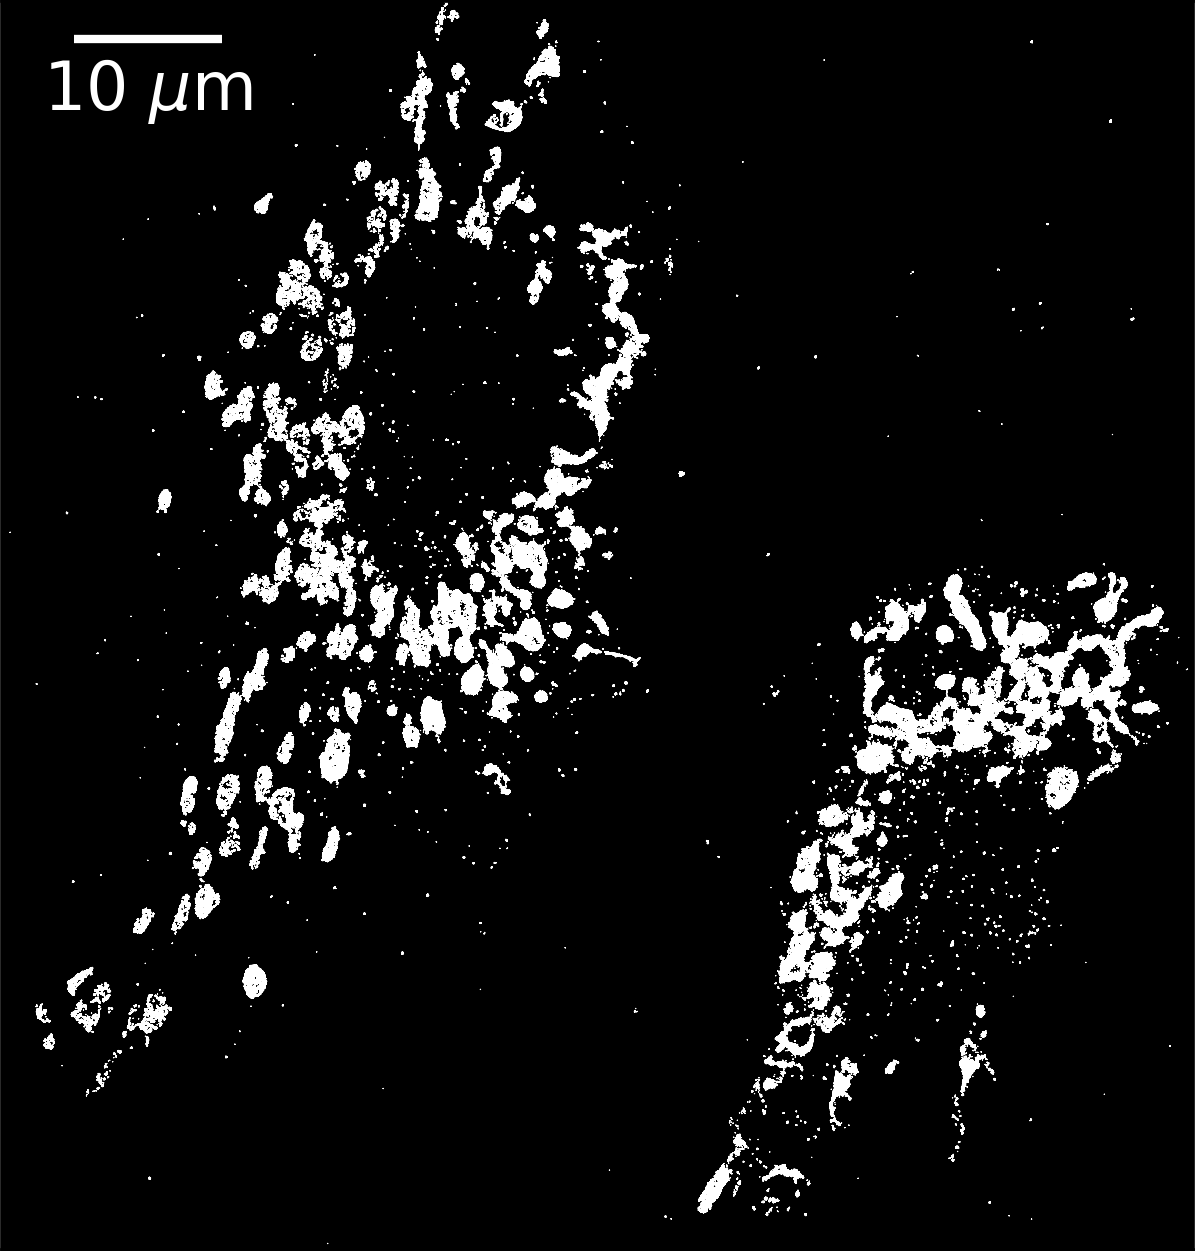
\includegraphics[width=\textwidth]{figures/mitochondria_image4.png}
        \caption{}
    \end{subfigure}
    \begin{subfigure}{0.32\textwidth}
        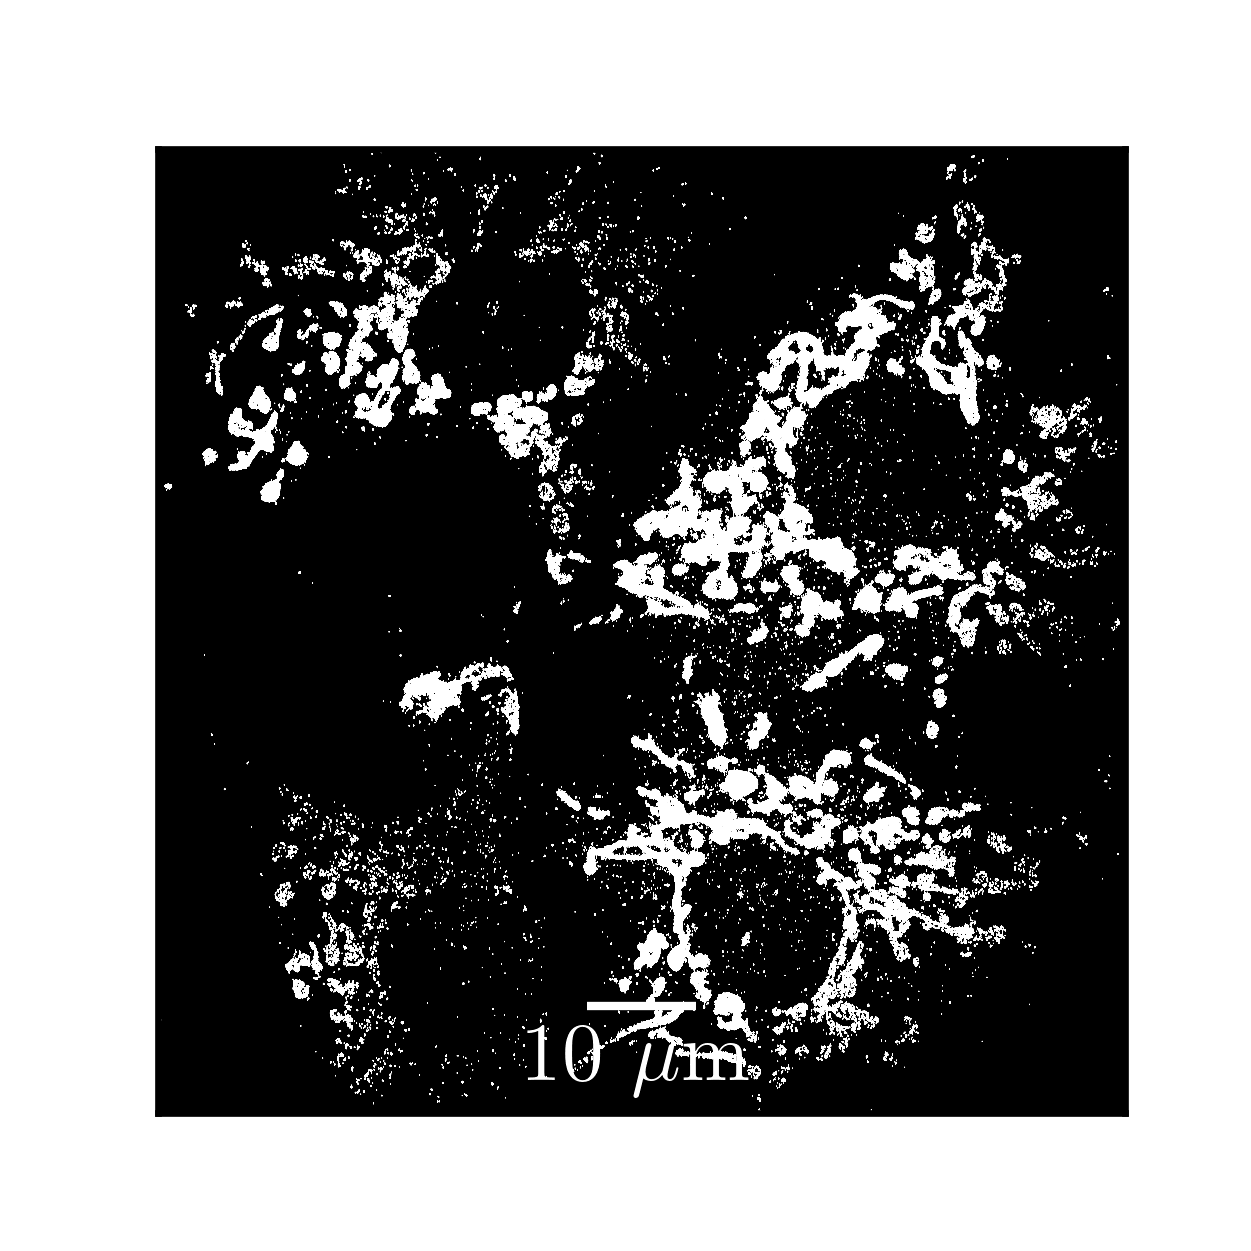
\includegraphics[width=\textwidth]{figures/mitochondria_image11.png}
        \caption{}
    \end{subfigure}
    \begin{subfigure}{0.32\textwidth}
        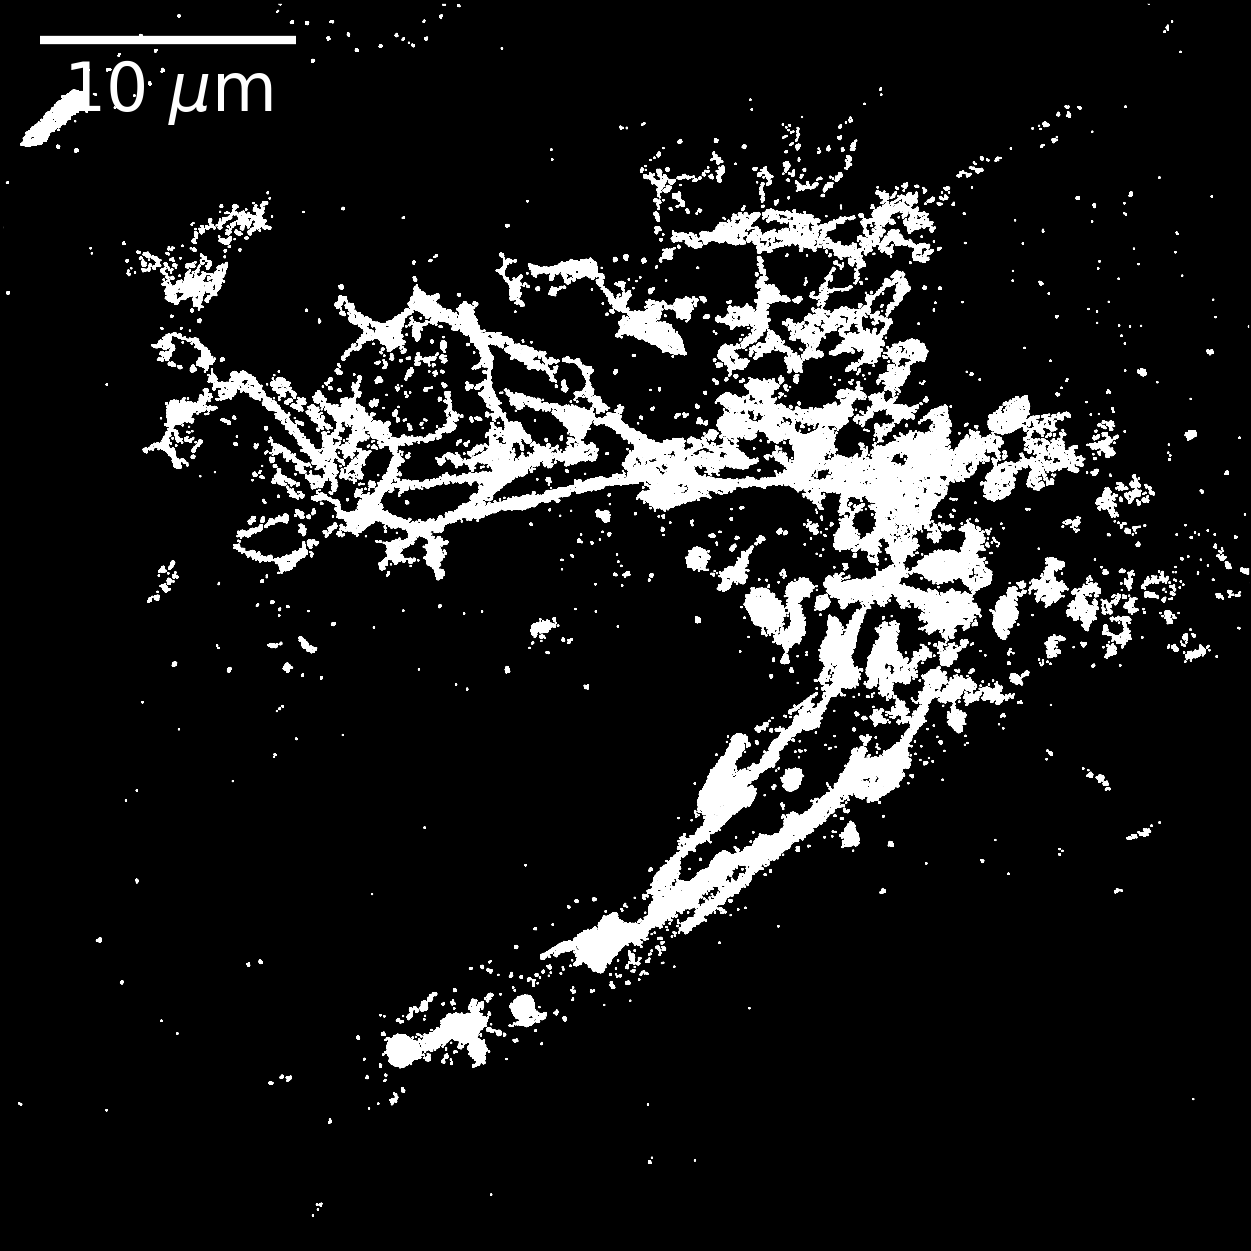
\includegraphics[width=\textwidth]{figures/mitochondria_image9.png}
        \caption{}
    \end{subfigure}
    \begin{subfigure}{0.32\textwidth}
        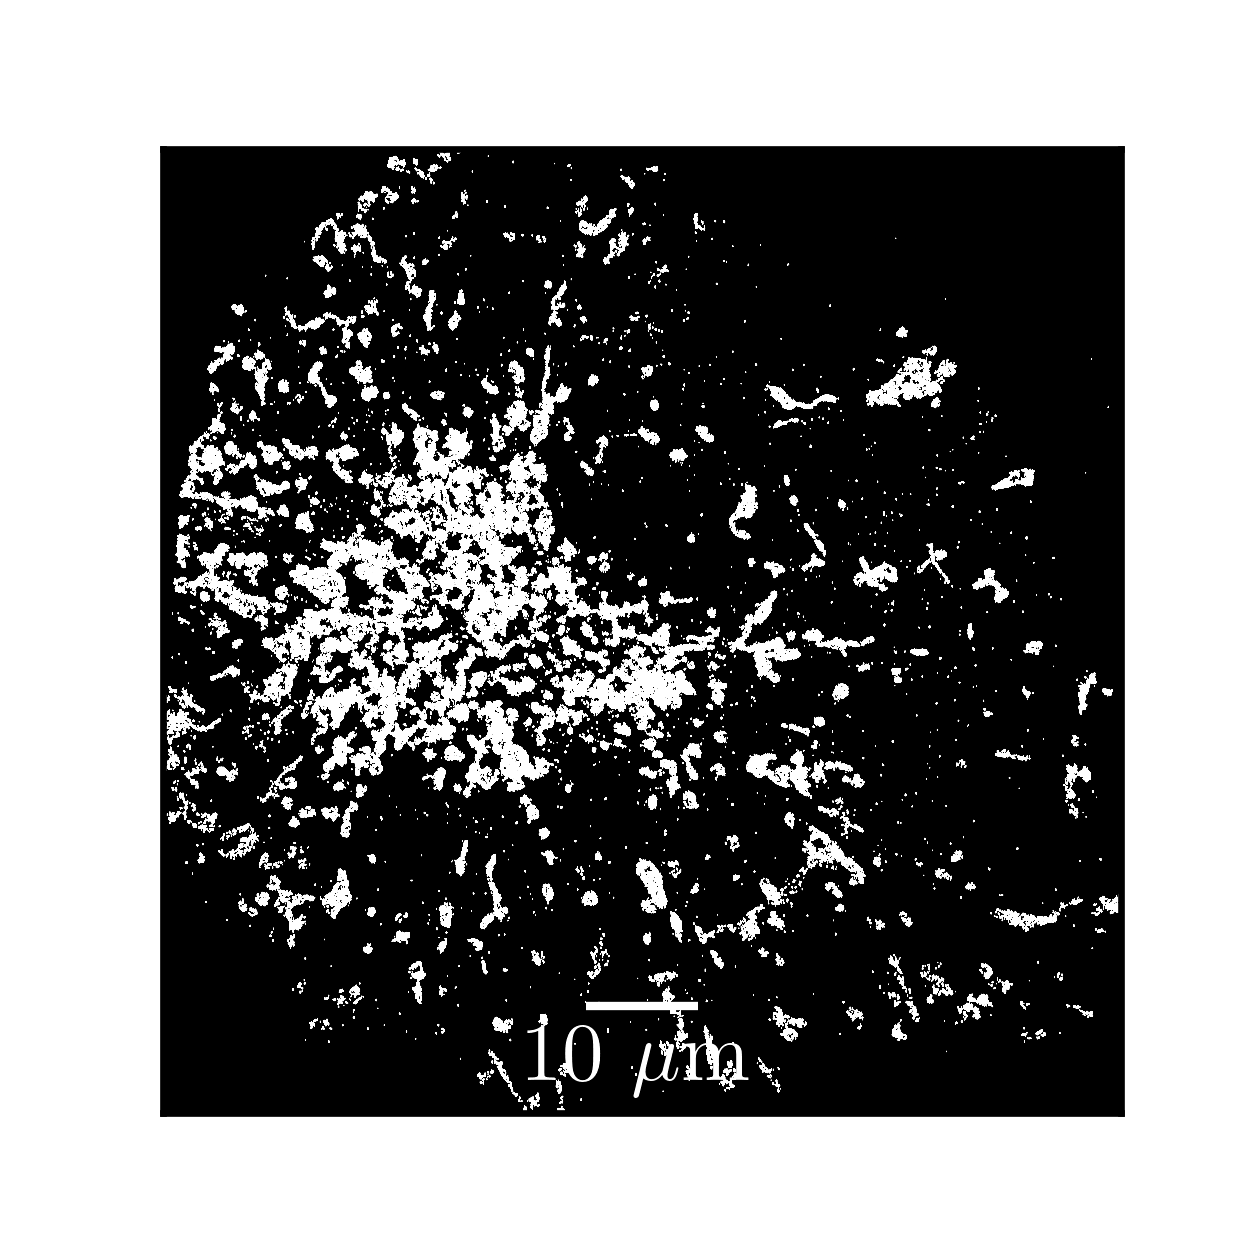
\includegraphics[width=\textwidth]{figures/mitochondria_image12.png}
        \caption{}
    \end{subfigure}
    \begin{subfigure}{0.32\textwidth}
        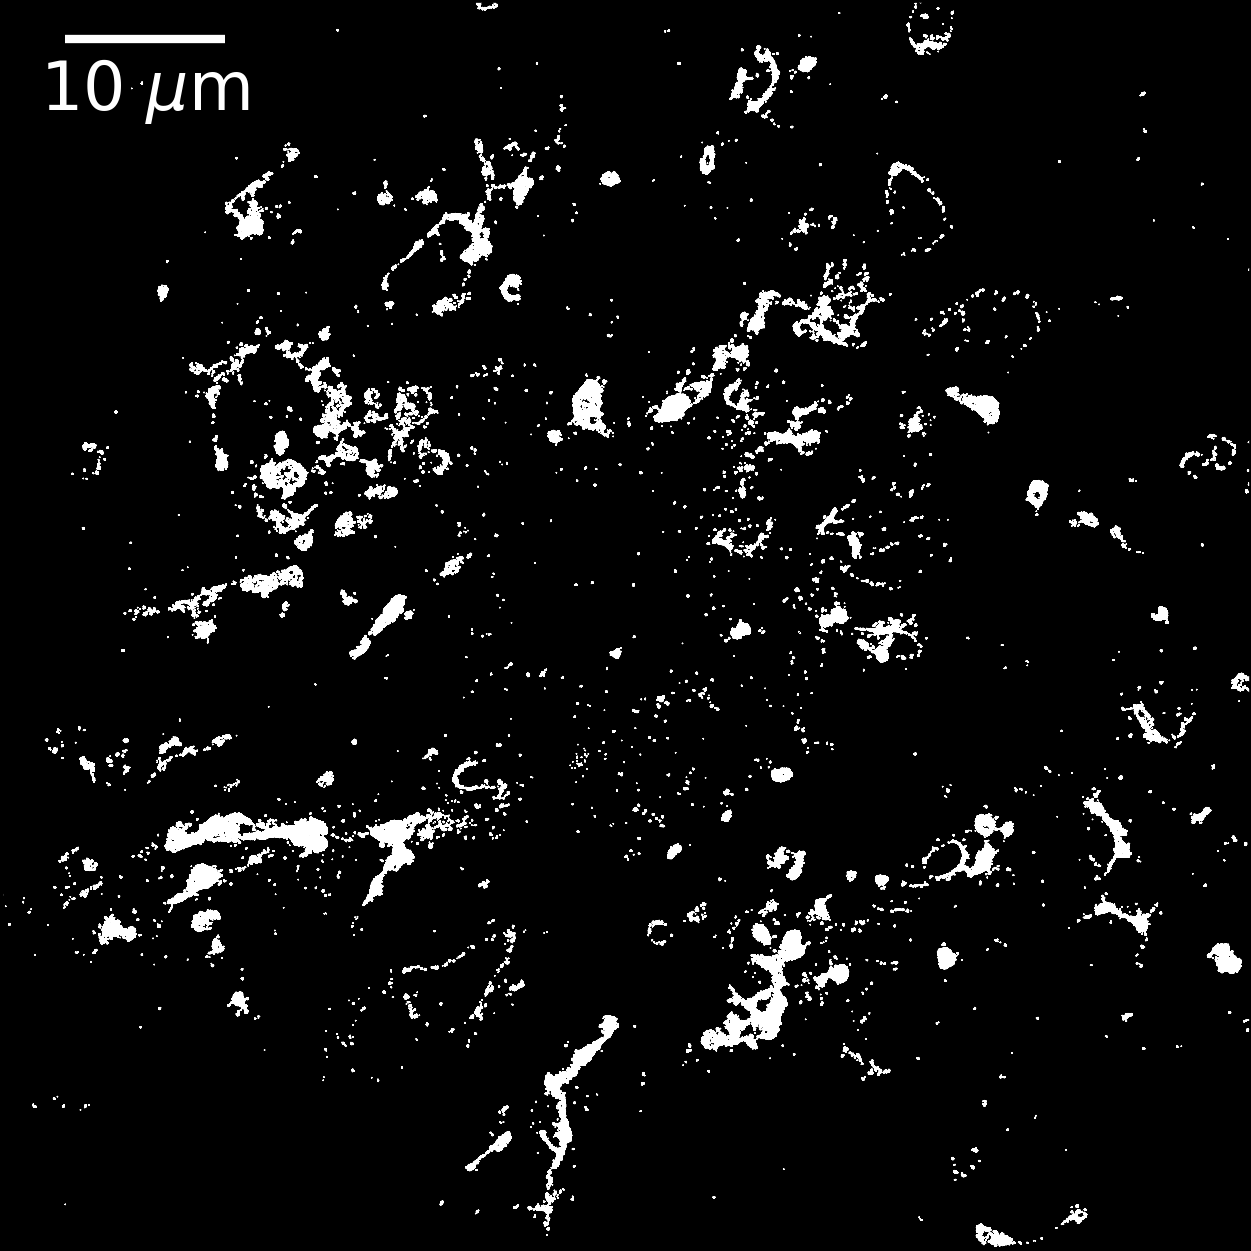
\includegraphics[width=\textwidth]{figures/mitochondria_image10.png}
        \caption{}
    \end{subfigure}
    \caption{Mitochondrial structures REDUIRE CONTRASTE}
\end{figure}